\subsection{Valutazione trajectory-aware}

La campagna D confronta Fixed FEM, la GNN statica A e il controller trajectory-aware nel solver ALE nativo. Per ogni caso sono condivisi stato iniziale, mesh, condizioni al contorno, $\Delta t=0.005$, $T=0.5$ e 100 passi; l'adattamento avviene ogni dieci passi. Non è applicato remapping esplicito. La Tabella~\ref{tab:staged_overall} riporta gli errori medi sui 28 casi held-out.

\begin{table*}[!t]
\centering\small
\caption{Errore relativo medio sui 28 casi held-out della campagna D. Valori percentuali; $\overline E_{L^2}$ è mediato nel tempo.}
\label{tab:staged_overall}
\begin{tabular*}{\textwidth}{@{\extracolsep{\fill}}lrrrr}
\toprule
Strategia & $\overline E_{L^2}$ & $E_{L^2}(T)$ & $\overline E_{|H^1|}$ & $E_{|H^1|}(T)$\\
\midrule
Fixed FEM & 10.633 & 11.735 & 32.618 & 33.388\\
GNN statica A + filtro & 11.478 & 13.355 & 34.700 & 37.035\\
GDM trajectory-aware D & \textbf{9.831} & \textbf{10.821} & \textbf{30.771} & \textbf{32.544}\\
\bottomrule
\end{tabular*}
\end{table*}

Il controller trajectory-aware riduce l'errore relativo $L^2$ integrato dal 10.633\% al 9.831\% e l'errore finale dall'11.735\% al 10.821\%. La riduzione media appaiata dell'endpoint primario è 8.038\%, con segno favorevole in tutti i 28 casi. Nei due split, l'errore integrato passa dall'8.729\% all'8.043\% in interpolazione e dal 12.060\% all'11.172\% in estrapolazione. La Figura~\ref{fig:staged_error_time} mostra l'andamento temporale medio nei due regimi.

\begin{figure*}[!t]
\centering
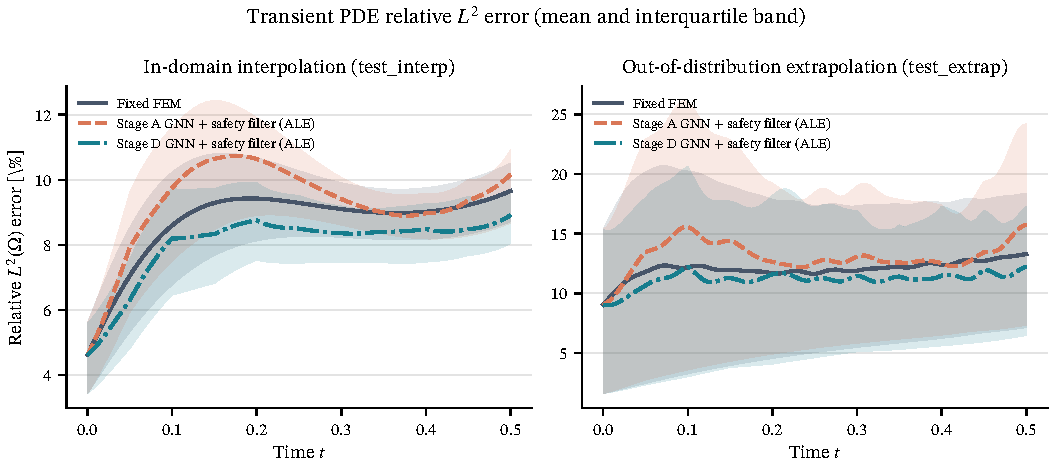
\includegraphics[width=0.92\textwidth,height=0.25\textheight,keepaspectratio]{images/stage_d/fig1_relative_l2_error_over_time.pdf}
\caption{Evoluzione temporale dell'errore relativo $L^2$ per Fixed FEM, GNN statica e GDM trajectory-aware, separata per i regimi interpolativo ed estrapolativo.}
\label{fig:staged_error_time}
\end{figure*}

L'errore in seminorma $H^1$ integrato favorisce mediamente il controller trajectory-aware, mentre l'errore finale $H^1$ non migliora in tutti i casi: nel totale la riduzione è positiva in 21/28 casi. La Tabella~\ref{tab:paired_stage_d} e il grafico appaiato completo sono collocati nell'Appendice~\ref{app:stage_d_audit} per mantenere distinto l'endpoint primario dalle metriche secondarie.

Le diagnostiche complete del filtro e della qualità geometrica sono riportate nella campagna F1 e nell'Appendice~\ref{app:stage_d_audit}.

La discrepanza $D_M$ non è un residuo di conservazione. La sua media relativa è circa $1.62\times10^{-4}$ per Fixed FEM e $6.36\times10^{-3}$ per GDM. Separatamente, il test D-GCL riportato nella Sezione~\ref{sec:stagee} riguarda la compatibilità geometrica della formulazione ALE.
